\documentclass[../main.tex]{subfiles}


\begin{document}

\section{Computer Boot Process}
\label{sec:computer-boot-process}

\subsection{Overview}

Upon powering up a computer, it undergoes a predetermined sequence of steps known as the \texttt{boot process}.
The boot process responsibilities encompass:
\begin{itemize}
  \item Locating and initializing hardware devices
  \item Loading and executing the operating system bootloader
  \item Providing configuration wizard for configuring onboarding devices
\end{itemize}

First step is to initialize the CPU and memory. Then CPU executes
code at a fixed memory location, known as the \texttt{reset vector}.
For \texttt{x86} architecture, the reset vector is at address \texttt{0xFFFFFFF0h} \cite{resetvector}.
At this address, a hardware flash memory known as \texttt{BIOS} is located (figure \ref{fig:uefi_chip}). \texttt{BIOS} is a firmware
that initializes the hardware and loads the bootloader. The bootloader is a small program that
loads the operating system kernel into memory and executes it. The operating system kernel
is the base component of operating system which manages the hardware and provides functions for
accessing the hardware.

On modern computers, the \texttt{BIOS} is replaced by \texttt{UEFI} (Unified Extensible Firmware Interface) \cite{uefi_spec}.
UEFI is a specification that defined a software interface between the operating system and the platform firmware.
It is designed to replace the \texttt{BIOS} firmware interface. \texttt{UEFI} is a more capable firmware which supports:
\begin{itemize}
  \item Secure boot
  \item Network boot \footnote{Network boot is a process of providing boot configuration and code over network}\footnote{It is also possible to network boot computer that uses BIOS}
  \item Booting from large disks \footnote{Larger than 2.2 TB \cite{bios_limits}}
  \item Booting from disks with GUID Partition Table (GPT)
  \item Booting from disks with more than 4 physical partitions
\end{itemize}

\begin{figure}[H]
  \centering
  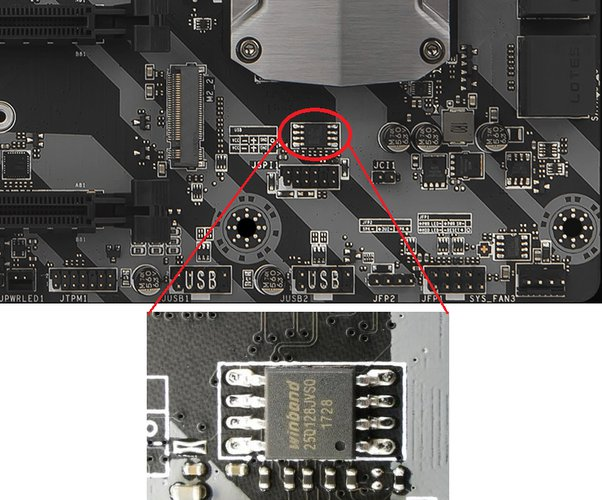
\includegraphics[width=\textwidth]{uefi_chip.jpg}
  \caption{Flash memory on motherboard containing UEFI firmware \cite{uefi_chip_img_ref}}
  \label{fig:uefi_chip}
\end{figure}

\end{document}